\chapter{THỰC NGHIỆM VÀ ĐÁNH GIÁ}

\section{Mô tả dữ liệu và môi trường thực nghiệm}

Để đảm bảo tính khách quan và khả năng ứng dụng thực tế, các thực nghiệm trong nghiên cứu này được tiến hành trên nền tảng đám mây với nguồn dữ liệu đa dạng và độc lập. Phần dưới đây mô tả chi tiết về cấu hình phần cứng, phần mềm và đặc tả các bộ dữ liệu được sử dụng.

\subsection{Môi trường thực nghiệm}
Toàn bộ quá trình huấn luyện và đánh giá được thực hiện trên nền tảng cloud \textbf{Vast.ai}, thuê GPU theo giờ để đảm bảo nguồn lực tính toán đủ mạnh cho training 3D.
\begin{itemize}
    \item \textbf{Phần cứng:} NVIDIA RTX 4090 (24GB VRAM), CUDA 12.x, $\sim$60GB RAM, ổ NVMe.
    \item \textbf{Framework:} PyTorch 2.0+, Python 3.10.
    \item \textbf{Thư viện chính:} SimpleITK, pydicom, OpenCV, scikit-learn, numpy.
\end{itemize}

\subsection{Tập dữ liệu RSNA 2024 Lumbar Spine Degenerative Classification \cite{rsna2024dataset}}
Đây là tập dữ liệu chủ đạo dùng để huấn luyện và đánh giá mô-đun grading. Bộ dữ liệu được tổ chức bởi Hiệp hội X-Quang Bắc Mỹ (RSNA) phối hợp cùng Hiệp hội Thần kinh học Hoa Kỳ (ASNR).

\begin{itemize}
    \item \textbf{Nguồn gốc và quy mô:} Dữ liệu được thu thập từ 8 trung tâm y tế lớn trên 5 châu lục, đảm bảo tính đa dạng về quần thể bệnh nhân và thiết bị chụp. Nhãn dữ liệu được gán thủ công bởi hơn 50 chuyên gia chẩn đoán hình ảnh. Train split $\sim$1\,800 patients (4 fold), val split $\sim$225 patients; mỗi patient có nhiều series MRI (Sagittal T2/STIR, Sagittal T1, Axial T2).
    \item \textbf{Đầu vào:} Ảnh MRI cột sống thắt lưng, định dạng chuẩn DICOM (mỗi series có hàng chục lát sagittal/axial). Quá trình tiền xử lý trích xuất \emph{khối ảnh đĩa đệm 3D} (per-IVD volume) quanh tâm mỗi đĩa đệm, resample về kích thước thống nhất $D \times H \times W = 9 \times 112 \times 224$ (float32), với $D = 9$ lát sagittal trung tâm theo chuẩn của SpineNetV2~\cite{windsor2022spinenetv2}, đủ bao phủ chiều dày đĩa đệm và mô lân cận, cân bằng giữa độ phủ giải phẫu và chi phí tính toán.
    \item \textbf{Nhãn bệnh lý:} Phân loại 5 tình trạng thoái hóa tại 5 tầng đĩa đệm (từ L1/L2 đến L5/S1):
        \begin{itemize}
            \item[$\circ$] Left Neural Foraminal Narrowing
            \item[$\circ$] Right Neural Foraminal Narrowing
            \item[$\circ$] Left Subarticular Stenosis
            \item[$\circ$] Right Subarticular Stenosis
            \item[$\circ$] Spinal Canal Stenosis
        \end{itemize}
    \item \textbf{Hệ thống phân cấp:} Mức độ nghiêm trọng được chia thành 3 cấp: Normal/Mild, Moderate, Severe.
    \item \textbf{Phân bố lớp (mất cân bằng):} Lớp Severe chỉ chiếm $\sim$4\% mẫu trong khi Normal/Mild chiếm $\sim$81\%, nguồn gốc bài toán mất cân bằng. Hình~\ref{fig:rsna_class_dist} minh họa chi tiết.
    \item \textbf{Vai trò trong nghiên cứu:} Training set chính + validation set để tinh chỉnh mô-đun grading và so sánh 4 cấu hình ablation.
\end{itemize}

\begin{figure}[H]
    \centering
    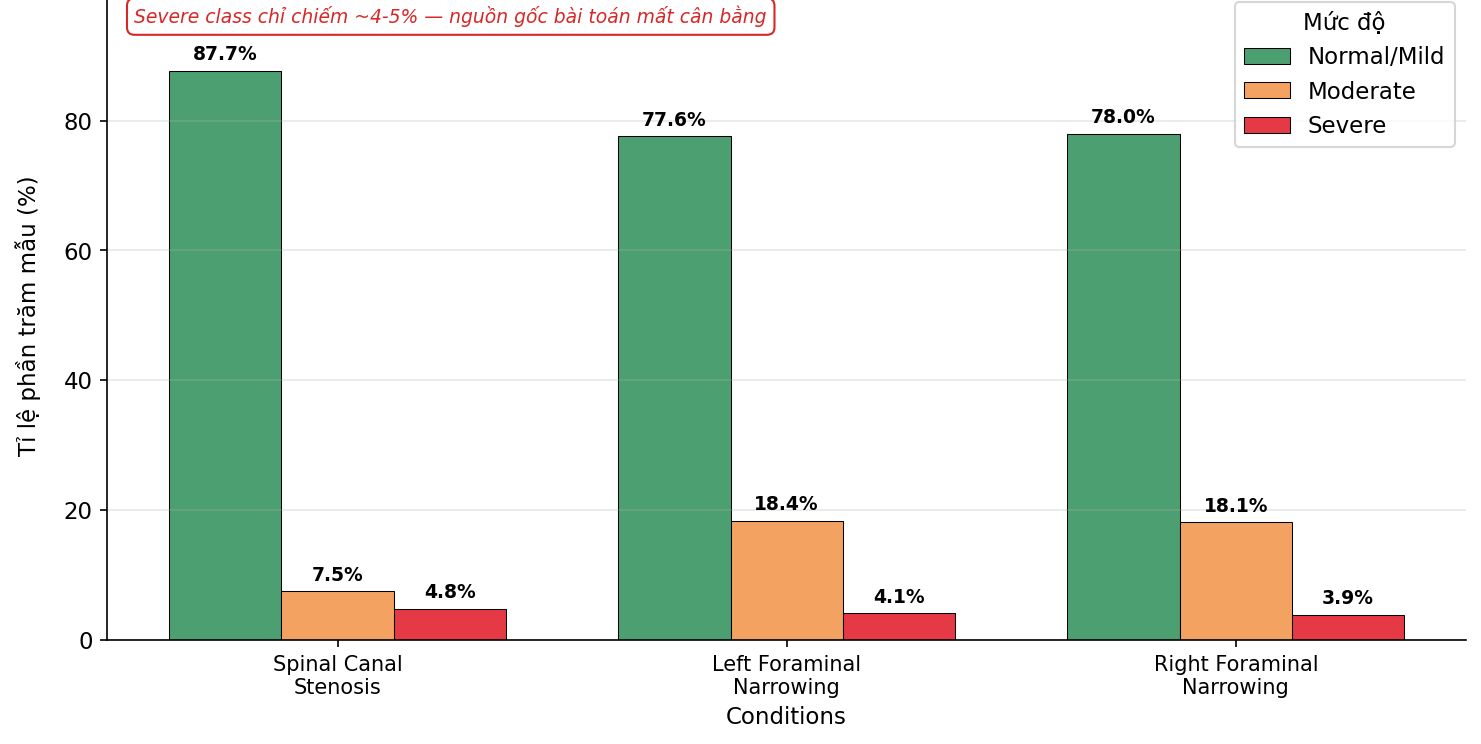
\includegraphics[width=0.95\textwidth]{cslt/rsna_class_distribution.png}
    \caption{Phân bố lớp trên RSNA 2024.}
    \label{fig:rsna_class_dist}
\end{figure}


\subsection{Tập dữ liệu Lumbar Spine Segmentation \cite{chu2015dataset}}
Tập dữ liệu được công bố bởi Chu và cộng sự \cite{chu2015dataset}, có nguồn gốc từ Viện Công nghệ và cơ sinh học phẫu thuật, Đại học Bern (Thụy Sĩ). Trong phạm vi báo cáo thực tập này, đây đóng vai trò là tập kiểm thử độc lập để đánh giá hiệu năng phân vùng của TotalSpineSeg.

\begin{itemize}
    \item \textbf{Quy mô:} Bao gồm ảnh MRI T2-weighted của 23 bệnh nhân ẩn danh. Mỗi ca chụp chứa ít nhất 7 thân đốt sống thuộc vùng cột sống dưới (từ T11 đến L5).
    \item \textbf{Đặc điểm hình ảnh:} Chuỗi xung Turbo Spin Echo trọng số T2. Dữ liệu được lưu trữ dưới định dạng NIfTI (.nii), giúp bảo toàn thông tin không gian 3D chuẩn y tế.
    \item \textbf{Nhãn phân vùng:}
        \begin{itemize}
            \item[$\circ$] \textbf{Loại nhãn:} Mặt nạ nhị phân.
            \item[$\circ$] \textbf{Đặc điểm:} Nhãn được gán cho toàn bộ vùng cột sống. Khác với các bộ dữ liệu hiện đại thường phân lớp chi tiết từng đốt sống, bộ dữ liệu này gán nhãn gộp cho cấu trúc đốt sống (bao gồm thân đốt sống và thành phần phụ) mà không tách biệt định danh từng đốt sống (L1, L2...).
        \end{itemize}
    \item \textbf{Mục đích sử dụng:} Đánh giá khả năng định vị và phân vùng cột sống trên miền dữ liệu chưa từng thấy, qua đó kiểm chứng độ bền vững của thuật toán phân vùng được chọn.
\end{itemize}

\subsection{Tập dữ liệu SPIDER \cite{vansluijs2022spider}}
Tập dữ liệu SPIDER (van der Graaf và cộng sự, công bố trên Nature Scientific Data 2024) được dùng làm test set độc lập để kiểm chứng khả năng tổng quát hóa cross-dataset của mô-đun grading.

\begin{itemize}
    \item \textbf{Quy mô:} 218 bệnh nhân $\times$ $\sim$5 đĩa đệm $\approx$ 1\,520 IVD samples, hoàn toàn độc lập với RSNA.
    \item \textbf{Định dạng:} Các file MetaImage \texttt{.mha} (đọc qua \texttt{SimpleITK}), kèm segmentation mask 3D với label 201--207 chỉ vị trí từng đĩa đệm.
    \item \textbf{Nhãn bệnh lý (mở rộng so với RSNA):} 8 nhãn theo chuẩn lâm sàng:
        \begin{itemize}
            \item[$\circ$] Pfirrmann grade (5 lớp): thang đo thoái hóa đĩa đệm.
            \item[$\circ$] Modic changes (4 lớp): biến đổi tủy xương dưới sụn.
            \item[$\circ$] Disc narrowing (binary): hẹp đĩa đệm.
            \item[$\circ$] Spondylolisthesis (binary): trượt đốt sống.
            \item[$\circ$] Upper/Lower endplate damage (binary $\times$ 2): tổn thương mặt trên/dưới đốt sống.
            \item[$\circ$] Disc herniation (binary): thoát vị đĩa đệm.
            \item[$\circ$] Disc bulging (binary): phồng đĩa đệm.
        \end{itemize}
    \item \textbf{Phân bố lớp:} Hai nhãn mất cân bằng nghiêm trọng là Spondylolisthesis (2.8\% positive) và Disc herniation (4.7\% positive). Chi tiết ở Hình~\ref{fig:spider_class_dist}.
    \item \textbf{Vai trò trong nghiên cứu:} Test set độc lập cho transfer learning, đánh giá: (i) mô hình huấn luyện trên RSNA có chuyển giao tốt sang dataset khác? (ii) các nhãn mới (Pfirrmann, Modic, \ldots) có học được từ feature backbone đã pretrained không?
\end{itemize}

\begin{figure}[H]
    \centering
    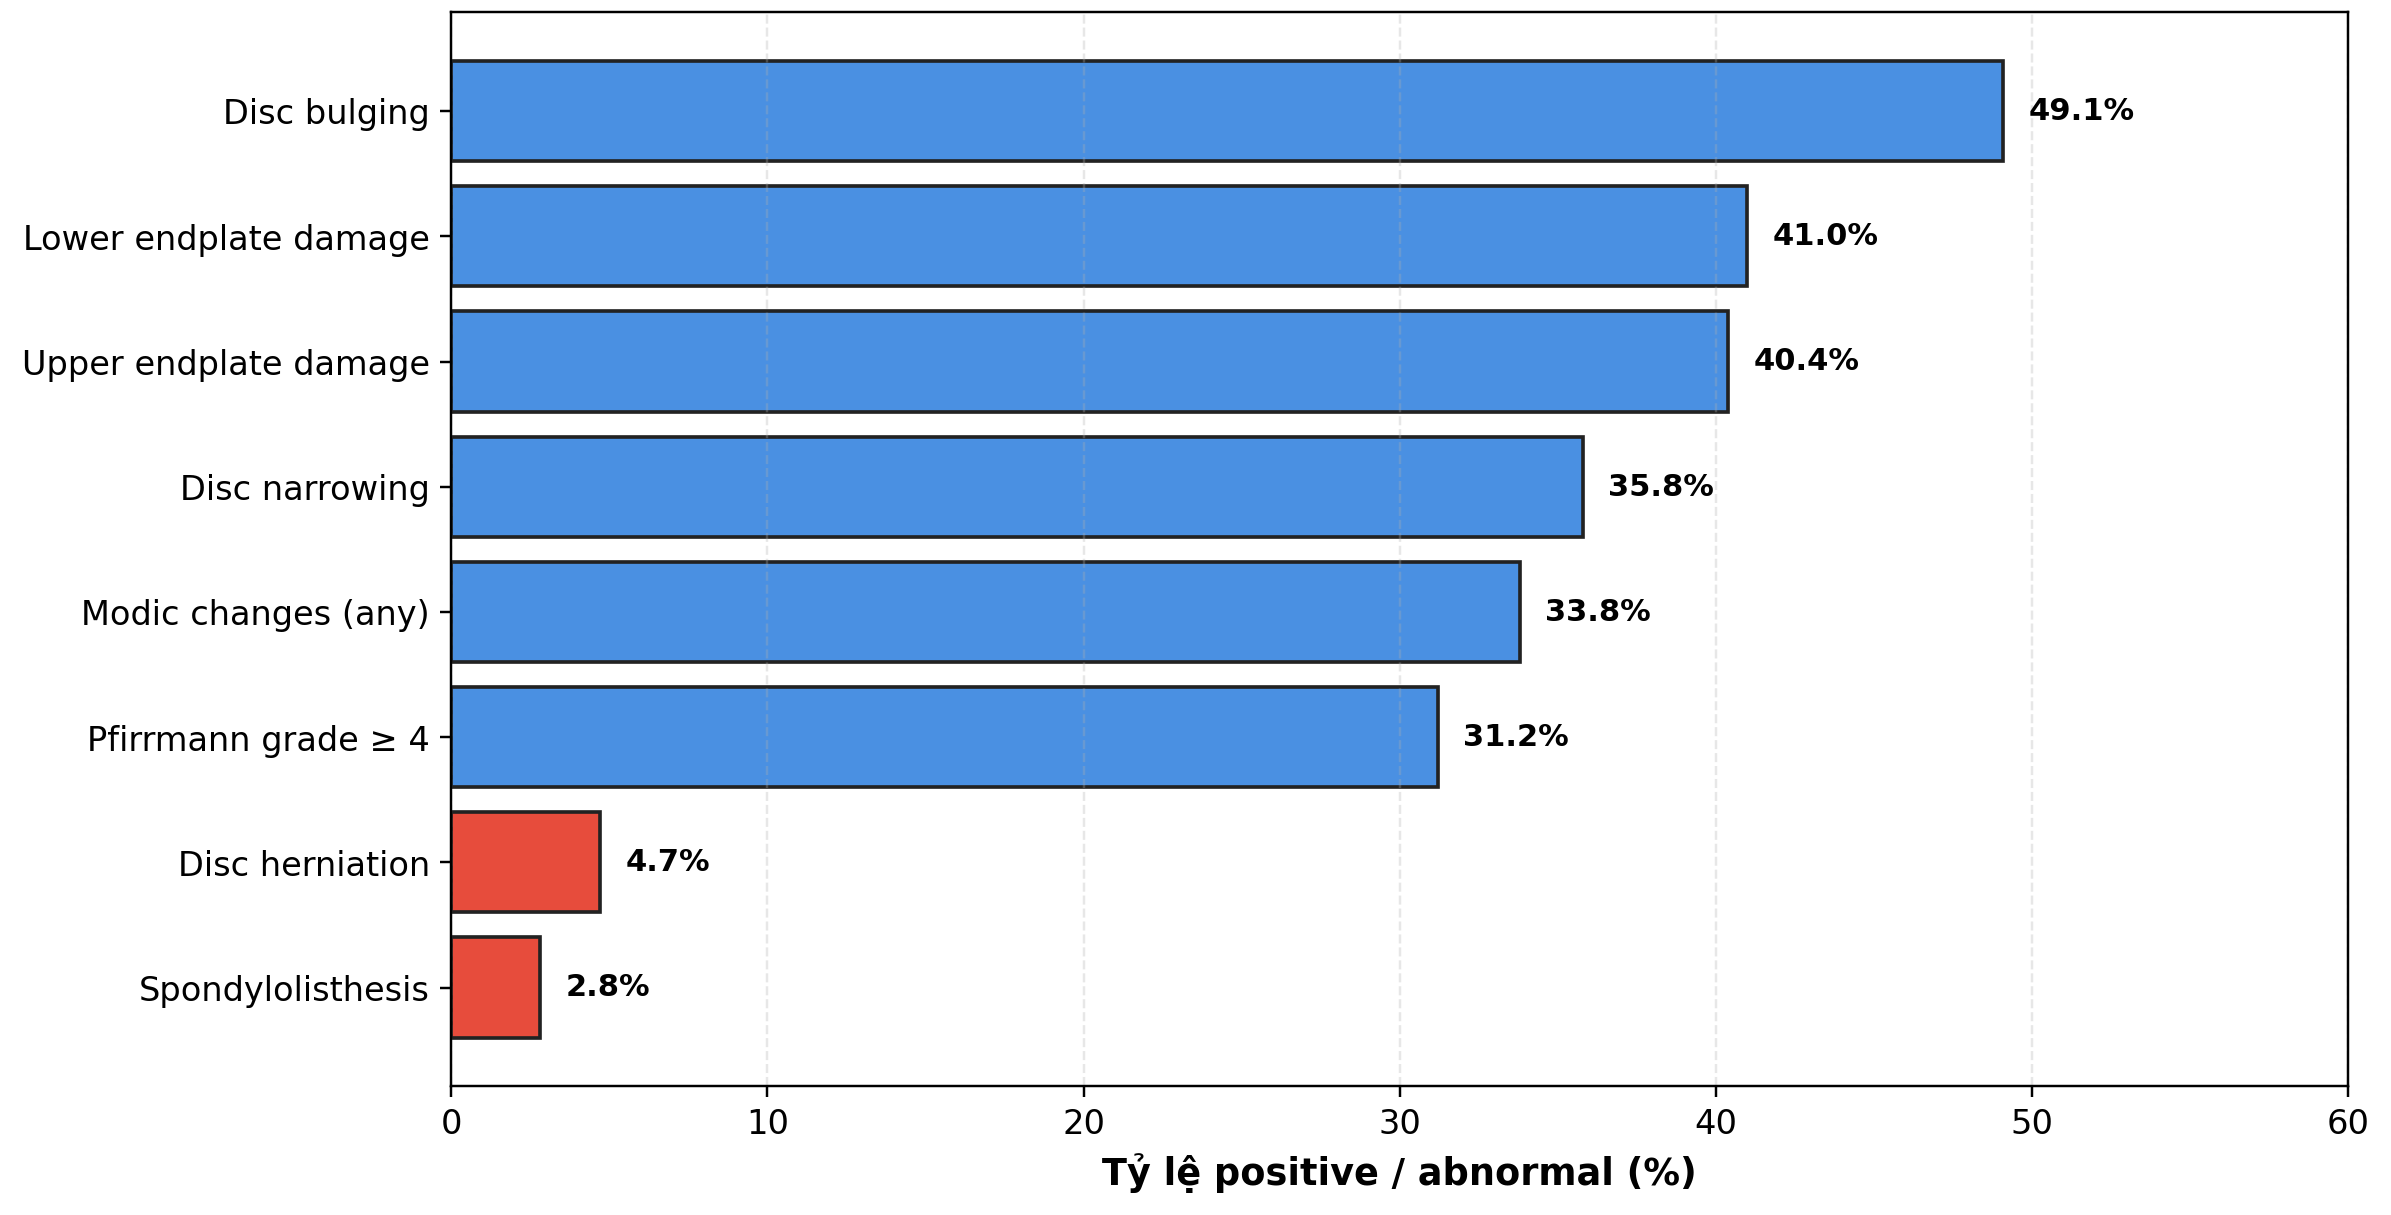
\includegraphics[width=\textwidth]{cslt/spider_class_distribution.png}
    \caption{Phân bố nhãn trên SPIDER 8 conditions.}
    \label{fig:spider_class_dist}
\end{figure}


\section[Thí nghiệm chọn mô-đun phân vùng]{Thí nghiệm chọn mô-đun phân vùng}
\label{sec:eval_segmentation}

\textbf{Mục tiêu thí nghiệm:} chọn 1 trong 4 mô hình phân vùng sẵn có cho pipeline đề xuất. Thí nghiệm so sánh \textbf{TotalSpineSeg} (tối ưu cho thân đốt sống), \textbf{SPINEPS} (tối ưu cho toàn bộ cấu trúc cột sống), \textbf{MedCLIP-SAMv2} (zero-shot text-driven), và \textbf{SpineNetV2} (mô hình spine chuyên dụng) trên tập kiểm thử 23 khối ảnh Ground Truth (vùng từ T11 đến L5).

\subsection{Các tiêu chí đánh giá}
Để đánh giá định lượng chất lượng phân vùng ảnh y tế 3D, nghiên cứu sử dụng các chỉ số tiêu chuẩn sau:

\begin{itemize}
    \item \textbf{Hệ số Dice (Dice Score):} 
    Thước đo phổ biến nhất về độ chồng lắp giữa vùng dự đoán ($P$) và nhãn thực tế ($G$) trong không gian 3D.
    \begin{equation}
        \text{Dice} = \frac{2 \times |P \cap G|}{|P| + |G|}
    \end{equation}

    \item \textbf{Chỉ số IoU (Jaccard Index):}
    Tỷ lệ giữa phần giao và phần hợp của hai tập hợp voxel.
    \begin{equation}
        \text{IoU} = \frac{|P \cap G|}{|P \cup G|}
    \end{equation}

    \item \textbf{Precision và Recall:}
    Đánh giá độ chính xác và độ bao phủ của mô hình.
    \begin{equation}
        \text{Precision} = \frac{TP}{TP + FP}, \quad \text{Recall} = \frac{TP}{TP + FN}
    \end{equation}
    \textit{Trong đó $TP$, $FP$, $FN$ lần lượt là số lượng voxel dự đoán đúng, dự đoán thừa và bỏ sót.}

    \item \textbf{Average Symmetric Surface Distance (ASSD):}
    Đây là chỉ số đánh giá độ sai lệch trung bình giữa bề mặt 3D của vùng dự đoán ($\partial P$) và bề mặt thực tế ($\partial G$). Chỉ số này được tính bằng trung bình cộng khoảng cách từ tất cả các điểm trên bề mặt dự đoán đến bề mặt thực tế và ngược lại.
    \begin{equation}
        \text{ASSD} = \frac{1}{|\partial P| + |\partial G|} \left( \sum_{p \in \partial P} d(p, \partial G) + \sum_{g \in \partial G} d(g, \partial P) \right)
    \end{equation}
    \textit{Trong đó $d(x, S)$ là khoảng cách Euclid ngắn nhất từ điểm $x$ đến bề mặt $S$ trong không gian 3 chiều. Giá trị ASSD càng nhỏ chứng tỏ bề mặt tái tạo càng chính xác.}
\end{itemize}

\subsection{Kết quả thực nghiệm}
Bảng \ref{tab:seg_results} trình bày kết quả so sánh trung bình trên 4 mô hình. \textbf{TotalSpineSeg} đạt hiệu năng tổng thể cao nhất với chỉ số Dice (70.81\%) và Precision (97.87\%). \textbf{SpineNetV2} đạt kết quả Dice Score 67.82\% và có chỉ số Recall cao nhất bảng (91.79\%). Đối với mô hình zero-shot \textbf{MedCLIP-SAMv2}, mặc dù Recall đạt mức cao nhưng độ chính xác biên dạng còn hạn chế.

\begin{table}[h!]
    \centering
    \caption{So sánh hiệu năng phân vùng giữa TotalSpineSeg, SPINEPS, MedCLIP-SAMv2 và SpineNetV2}
    \label{tab:seg_results}
    \renewcommand{\arraystretch}{1.2}
    \setlength{\tabcolsep}{4pt}
    \begin{tabular}{lcccc}
        \toprule
        \textbf{Tiêu chí} & \textbf{TotalSpineSeg} & \textbf{SPINEPS} & \textbf{MedCLIP-SAMv2} & \textbf{SpineNetV2} \\
        \midrule
        \textbf{Dice Score} & \textbf{70.81\%} & 58.68\% & 40.55\% & 67.82\% \\
        \textbf{IoU} & \textbf{55.74\%} & 41.56\% & 26.47\% & 51.41\% \\
        \textbf{Precision}  & \textbf{97.87\%} & 52.17\% & 29.16\% & 51.76\% \\
        \textbf{Recall}  & 56.49\% & 68.34\% & \textbf{91.98\%} & 91.79\% \\
        \textbf{ASSD}  & \textbf{6.85 mm} & 7.48 mm & 19.50 mm & 8.04 mm \\
        \bottomrule
    \end{tabular}
\end{table}

\subsection{Phân tích và thảo luận}

\subsubsection{Lý giải sự chênh lệch giữa Recall và Precision}
Kết quả thực nghiệm cho thấy sự khác biệt về đặc tính của từng mô hình, xuất phát từ thiết kế và định nghĩa nhãn thực tế:

\begin{itemize}
    \item \textbf{Vấn đề về ground truth:} Dữ liệu ground truth bao gồm toàn bộ đốt sống (thân + gai sau + mỏm ngang).
    \item \textbf{TotalSpineSeg:} Được thiết kế tập trung vào \textbf{thân đốt sống}, do đó mô hình chủ động bỏ qua các phần gai sau, dẫn đến Recall ở mức 56.49\%. Tuy nhiên, độ chính xác trên vùng thân đốt sống đạt mức rất cao (Precision 97.87\%) và ít nhiễu.
    \item \textbf{SpineNetV2:} Đạt chỉ số Recall 91.79\% nhờ chiến lược tối đa hóa vùng bao phủ. Mô hình có xu hướng tạo ra vùng dự đoán rộng để đảm bảo độ chồng lấn cao nhất với dữ liệu nhãn, ưu tiên việc phát hiện đầy đủ đối tượng hơn là tối ưu hóa biên dạng giải phẫu chi tiết như các mô hình phân vùng chuyên biệt.
    \item \textbf{SPINEPS \& MedCLIP-SAMv2:} Cả hai mô hình đều có Precision thấp (dưới 53\%), cho thấy hiện tượng phân vùng thừa (over-segmentation) so với nhãn mục tiêu. Riêng MedCLIP-SAMv2 có sai số biên dạng lớn nhất (ASSD 19.50mm).
\end{itemize}
\subsubsection{Lựa chọn mô hình cho hệ thống đề xuất}
Dựa trên mục tiêu xây dựng hệ thống hỗ trợ chẩn đoán (yêu cầu xác định chính xác vị trí thân đốt sống để trích xuất ảnh), nghiên cứu lựa chọn \textbf{TotalSpineSeg} vì các lý do sau:

\begin{enumerate}
    \item \textbf{Độ tin cậy cao:} Precision 97.87\% đảm bảo vùng được xác định là đốt sống với độ chính xác cao, hạn chế nhiễu trong các bước xử lý tiếp theo, cao hơn đáng kể so với mức ~51\% của SpineNetV2 và SPINEPS.
    \item \textbf{Độ chính xác bề mặt 3D:} Chỉ số ASSD thấp (6.85mm) cho thấy khả năng tái tạo bề mặt thân đốt sống bám sát giải phẫu thực tế, tốt hơn so với MedCLIP-SAMv2 và SPINEPS.
    \item \textbf{Tính ổn định:} Độ lệch chuẩn thấp ($\pm 5.23\%$) cho thấy sự ổn định khi áp dụng trên dữ liệu lâm sàng. Mặc dù SpineNetV2 có Recall tốt hơn, nhưng Precision thấp khiến mô hình này phù hợp hơn cho bài toán phát hiện thay vì phân vùng chính xác cho phẫu thuật.
\end{enumerate}


\section{Thí nghiệm chọn mô-đun đánh giá phát hiện bất thường}
\label{sec:eval_detection}

\textbf{Mục tiêu thí nghiệm:} Chọn 1 trong 3 mô hình sẵn có làm backbone cho mô-đun grading trong pipeline đề xuất. Thí nghiệm so sánh các mô hình ở góc nhìn binary detection (có/không bệnh) trên RSNA val 150 bệnh nhân để xác định: (i) mô hình nào đủ chính xác và ổn định cho clinical screening, (ii) mô hình nào có kiến trúc đủ đơn giản và mã nguồn mở để có thể tinh chỉnh tiếp ở thí nghiệm xác thực đóng góp (Mục~\ref{sec:phase2_eval}).

Thực nghiệm được tiến hành so sánh giữa ba mô hình đại diện:
\begin{itemize}
    \item \textbf{SpineNetV2:} Mô hình mã nguồn mở với khả năng gán nhãn đa dạng (9-10 clinical features).
    \item \textbf{MedGemma:} Mô hình ngôn ngữ - thị giác lớn (VLM).
    \item \textbf{Ning Shen:} Giải pháp đạt giải nhất cuộc thi RSNA 2024 (SOTA Baseline).
\end{itemize}
\subsection{Các tiêu chí đánh giá}
Để đánh giá hiệu năng của các mô hình trên tập dữ liệu RSNA 2024 (bao gồm 150 bệnh nhân), nghiên cứu sử dụng các chỉ số phổ biến trong bài toán phân loại y tế: Accuracy, Precision, Recall và F1-Score.

Gọi $TP$ (True Positive) là số mẫu dương tính được dự đoán đúng, $TN$ (True Negative) là số mẫu âm tính được dự đoán đúng, $FP$ (False Positive) là số mẫu âm tính bị dự đoán sai thành dương tính, và $FN$ (False Negative) là số mẫu dương tính bị dự đoán sai thành âm tính. Các công thức được định nghĩa như sau:

\begin{equation}
    \text{Accuracy} = \frac{TP + TN}{TP + TN + FP + FN}
\end{equation}

\begin{equation}
    \text{Precision} = \frac{TP}{TP + FP}
\end{equation}

\begin{equation}
    \text{Recall} = \frac{TP}{TP + FN}
\end{equation}

\begin{equation}
    \text{F1-Score} = 2 \times \frac{\text{Precision} \times \text{Recall}}{\text{Precision} + \text{Recall}}
\end{equation}

\textbf{Per-class F1 (Severe F1, Moderate F1, Normal F1).} Khi bài toán có nhiều lớp (Normal/Mild, Moderate, Severe), 4 chỉ số ở trên có thể tính \emph{riêng cho từng lớp} (theo cách one-vs-rest). Ví dụ \textit{Severe F1} chỉ tính trên các mẫu thuộc lớp Severe --- đặc biệt quan trọng cho bài toán mất cân bằng vì class hiếm dễ bị ``che lấp'' bởi class chiếm đa số.

\textbf{Mean F1 macro.} Trung bình cộng F1 trên tất cả các lớp, mỗi lớp có trọng số bằng nhau:
\begin{equation}
    \text{F1}_{\text{macro}} = \frac{1}{K} \sum_{k=1}^{K} \text{F1}_k
\end{equation}
với $K$ là số lớp. Khác với F1 weighted (lấy trung bình theo tần suất class), F1 macro \emph{phạt mạnh các class hiếm có hiệu năng thấp}, phù hợp cho clinical screening vì các ca Severe quan trọng nhưng số lượng ít.

\textbf{AUC (Area Under ROC Curve).} Diện tích dưới đường cong ROC, biểu diễn quan hệ giữa True Positive Rate (Recall) và False Positive Rate khi thay đổi ngưỡng quyết định. AUC = 0.5 tương đương dự đoán ngẫu nhiên, AUC = 1.0 là phân loại hoàn hảo. \emph{Ưu điểm:} không phụ thuộc ngưỡng phân loại, đánh giá chất lượng ranking của xác suất dự đoán.
\begin{equation}
    \text{AUC} = \int_0^1 \text{TPR}(\text{FPR}^{-1}(t)) \, dt
\end{equation}

\textbf{AUPRC (Area Under Precision-Recall Curve).} Diện tích dưới đường cong Precision-Recall. Phù hợp hơn AUC cho dữ liệu \emph{mất cân bằng nghiêm trọng}: AUC có thể trông cao một cách giả tạo khi class majority quá lớn, trong khi AUPRC tập trung vào hiệu năng của class hiếm (positive class). Báo cáo sử dụng AUPRC làm chỉ số chính cho lớp Severe.
\begin{equation}
    \text{AUPRC} = \int_0^1 \text{Precision}(\text{Recall}^{-1}(t)) \, dt
\end{equation}

\subsection{Kết quả thực nghiệm}

Ba mô hình được đánh giá trên tập validation gồm 150 bệnh nhân, bao gồm ba nhóm bệnh lý chính: Hẹp ống sống, hẹp lỗ liên hợp trái, và hẹp lỗ liên hợp phải. Các chỉ số precision, recall, và F1-score được sử dụng để đánh giá khả năng phát hiện bất thường của từng mô hình.

\textbf{a. Hẹp ống sống}

Bảng~\ref{tab:scs_metrics} trình bày chi tiết kết quả của nhóm này. Kết quả cho thấy đây là nhóm bệnh lý có tỷ lệ phát hiện tốt nhất. Ning Shen đạt F1-Score 81.20\% với precision 81.82\% và recall 80.60\%, cho thấy model này phát hiện khá chính xác và ít bỏ sót. SpineNetV2 đạt F1-Score 78.79\% với recall 80.00\%, cũng thể hiện khả năng phát hiện tốt. MedGemma có F1-Score thấp hơn nhiều (31.17\%) do recall chỉ 20.87\%, nghĩa là bỏ sót gần 80\% bệnh nhân có bệnh hẹp ống sống.

\begin{table}[h!]
    \centering
    \caption{Kết quả chi tiết nhóm Hẹp ống sống}
    \label{tab:scs_metrics}
    \renewcommand{\arraystretch}{1.2}
    \begin{tabular}{lcccc}
        \toprule
        \textbf{Mô hình} & \textbf{Accuracy} & \textbf{Precision} & \textbf{Recall} & \textbf{F1-Score} \\
        \midrule
        Ning Shen & \textbf{86.63\%} & \textbf{81.82\%} & \textbf{80.60\%} & \textbf{81.20\%} \\
        SpineNetV2 & 81.58\% & 77.61\% & 80.00\% & 78.79\% \\
        MedGemma & 29.33\% & 61.54\% & 20.87\% & 31.17\% \\
        \bottomrule
    \end{tabular}
\end{table}

\textbf{b. Hẹp lỗ liên hợp trái}

Bảng~\ref{tab:nfn_left_metrics} trình bày chi tiết kết quả của nhóm này. Ning Shen đạt F1-Score 79.43\% với Recall cao (87.37\%), phù hợp với yêu cầu của screening là cần ưu tiên phát hiện được nhiều trường hợp bị bệnh. SpineNetV2 cũng có Recall cao (84.00\%) và F1-Score 77.30\%, cho thấy sự cân bằng khá tốt giữa khả năng phát hiện và độ chính xác. MedGemma có hiệu năng kém hơn với F1-Score 13.86\% do Recall chỉ 8.43\%, tức là bỏ sót hơn 91\% bệnh nhân bị bệnh Hẹp lỗ liên hợp trái.

\begin{table}[h!]
    \centering
    \caption{Kết quả chi tiết nhóm Hẹp lỗ liên hợp trái}
    \label{tab:nfn_left_metrics}
    \renewcommand{\arraystretch}{1.2}
    \begin{tabular}{lcccc}
        \toprule
        \textbf{Mô hình} & \textbf{Accuracy} & \textbf{Precision} & \textbf{Recall} & \textbf{F1-Score} \\
        \midrule
        Ning Shen & \textbf{77.01\%} & \textbf{72.81\%} & \textbf{87.37\%} & \textbf{79.43\%} \\
        SpineNetV2 & 75.66\% & 71.59\% & 84.00\% & 77.30\% \\
        MedGemma & 42.00\% & 38.89\% & 8.43\% & 13.86\% \\
        \bottomrule
    \end{tabular}
\end{table}

\textbf{c. Hẹp lỗ liên hợp phải}

Bảng~\ref{tab:nfn_right_metrics} trình bày chi tiết kết quả của nhóm này. Ning Shen có F1-Score 81.48\% và Recall 84.62\%, thể hiện sự ổn định trên các nhóm bệnh lý khác nhau. SpineNetV2 đạt F1-Score 76.40\% với Precision và Recall khá cân bằng (75.56\% và 77.27\%). MedGemma có kết quả thấp nhất với F1-Score 10.75\% và Recall cực kỳ thấp (6.02\%), bỏ sót gần 94\% bệnh nhân bị Hẹp lỗ liên hợp phải. Điều này chứng tỏ MedGemma có xu hướng dự đoán quá an toàn (thiên về kết quả bình thường), do đó không đáp ứng được yêu cầu của việc sàng lọc

\begin{table}[h!]
    \centering
    \caption{Kết quả chi tiết nhóm Hẹp lỗ liên hợp phải}
    \label{tab:nfn_right_metrics}
    \renewcommand{\arraystretch}{1.2}
    \begin{tabular}{lcccc}
        \toprule
        \textbf{Mô hình} & \textbf{Accuracy} & \textbf{Precision} & \textbf{Recall} & \textbf{F1-Score} \\
        \midrule
        Ning Shen & \textbf{78.61\%} & \textbf{78.57\%} & \textbf{84.62\%} & \textbf{81.48\%} \\
        SpineNetV2 & 72.37\% & 75.56\% & 77.27\% & 76.40\% \\
        MedGemma & 44.67\% & 50.00\% & 6.02\% & 10.75\% \\
        \bottomrule
    \end{tabular}
\end{table}

\subsection{Phân tích và thảo luận}

\textbf{Hiệu năng: }Nhìn chung, Ning Shen có hiệu năng tốt nhất với F1-Score trung bình 80.37\% và khá ổn định trên cả ba nhóm bệnh lý (từ 79.43\% đến 81.48\%). Kết quả này phù hợp với kỳ vọng từ một SOTA model được thiết kế riêng cho RSNA 2024 dataset. SpineNetV2 đạt F1-Score trung bình 77.50\%, thấp hơn Ning Shen khoảng 3\%, nhưng vẫn cho thấy khả năng detection khá tốt với performance ổn định (76.40\% - 78.79\%). MedGemma có F1-Score trung bình thấp nhất (18.59\%), chủ yếu do Recall quá thấp (6.02\% - 20.87\%) ở tất cả các conditions. \\

\textbf{Về recall và precision trong bài toán sàng lọc}: 
Kết quả thực nghiệm cho thấy một xu hướng rõ rệt ở NingShen và SpineNetV2 là việc ưu tiên độ nhạy (Recall, đạt $80-87\%$) hơn so với độ chính xác (Precision, đạt $72-82\%$). Chiến lược này hoàn toàn phù hợp với nguyên tắc cốt lõi của bài toán sàng lọc y tế: tối thiểu hóa tỷ lệ bỏ sót bệnh (False negatives) ngay cả khi phải chấp nhận gia tăng tỷ lệ báo động giả (False positives). Trong thực tế lâm sàng, các cảnh báo giả có thể dễ dàng được bác sĩ loại bỏ qua quá trình kiểm tra chi tiết, nhưng việc bỏ sót một bệnh nhân có bệnh lại gây ra hậu quả nghiêm trọng hơn nhiều.\\

Trái lại, MedGemma thể hiện chiến lược dự đoán thận trọng quá mức. Mặc dù chỉ số Precision đạt mức chấp nhận được ($38.89\% - 61.54\%$), chỉ số Recall lại cực thấp ($6.02\% - 20.87\%$), đồng nghĩa với việc mô hình đã bỏ sót tới $80-94\%$ số ca bệnh thực tế. Điều này khẳng định rằng MedGemma, với bản chất là một mô hình VLM đa dụng chưa được tinh chỉnh cho dữ liệu cột sống thắt lưng, do đó không đáp ứng được yêu cầu của tác vụ sàng lọc.\\

\textbf{Độ ổn định giữa các nhóm bệnh:} Ning Shen có độ ổn định cao với F1-Score dao động ít (81.20\% - 81.48\% cho hai bệnh Hẹp lỗ liên hợp phải, hẹp ống sống, 79.43\% cho hẹp lỗ liên hợp trái). SpineNetV2 cũng khá ổn định (76.40\% - 78.79\%). Ngược lại, MedGemma có variance cao (10.75\% - 31.17\%), cho thấy performance không đồng đều và đặc biệt kém với Hẹp lỗ liên hợp phải. \\

\textbf{Mô hình được chọn:} \textbf{SpineNetV2} được chọn làm backbone cho mô-đun grading vì cân bằng tốt nhất giữa độ chính xác (F1 trung bình 77.50\%, chỉ thấp hơn Ning Shen 3\%) và tính khả thi triển khai (mã nguồn mở, kiến trúc 3D ResNet-34 đơn giản, dễ tinh chỉnh). Ning Shen có F1 cao hơn nhưng là ensemble nhiều mô hình lớn, khó duy trì và không phù hợp với pipeline thực tế của báo cáo. MedGemma bị loại do Recall quá thấp (6--21\%). \\

 Khi phân tích sâu hơn theo từng \emph{cấp độ bệnh} trên full RSNA, SpineNetV2 baseline có Severe Recall chỉ 11.5\%, gần 9/10 ca nặng bị bỏ sót, mặc dù detection-level F1 vẫn 77.50\%. Điểm yếu này là động cơ trực tiếp cho thí nghiệm tiếp theo: tinh chỉnh mô-đun grading bằng CBAM + BiomedCLIP để cải thiện cụ thể trên Severe class.

\section[Thí nghiệm xác thực đóng góp tinh chỉnh]{Thí nghiệm xác thực đóng góp tinh chỉnh}
\label{sec:phase2_eval}

{Mục tiêu thí nghiệm nhằm xác thực rằng các đóng góp tinh chỉnh (CBAM attention + BiomedCLIP frozen + pipeline xử lý mất cân bằng) thật sự cải thiện hiệu năng so với backbone đã chọn ở Mục~\ref{sec:eval_detection}. Thí nghiệm dựng 4 cấu hình ablation (SpineNetV2 / +CBAM / BMC-only / Hybrid) trên RSNA 2024 full train+val, đồng thời kiểm chứng tổng quát hóa qua transfer learning sang SPIDER 8-label với 3-seed evaluation.


\subsection{Thiết lập huấn luyện}
Toàn bộ thực nghiệm chạy trên NVIDIA RTX 4090 (24GB VRAM) trên Vast.ai cloud instance. Framework PyTorch 2.0+, Python 3.10.

% \begin{table}[h!]
% \centering
% \caption{Hyperparameter 4 cấu hình ablation.}
% \label{tab:phase2_hyperparams}
% \renewcommand{\arraystretch}{1.2}
% \setlength{\tabcolsep}{4pt}
% \begin{tabular}{lcccc}
% \toprule
% \textbf{Hyperparameter} & \textbf{SpineNetV2} & \textbf{CBAM} & \textbf{BMC-only} & \textbf{Hybrid} \\
% \midrule
% Optimizer & AdamW & AdamW & AdamW & AdamW \\
% Learning rate & 1e-3 & 1e-3 & 1e-3 & 1e-3 \\
% Batch size & 32 & 32 & 32 & 32 \\
% Epochs (RSNA) & 30 & 20 & 25 & 25 \\
% Augmentation & medium & medium & medium & medium \\
% Oversample factor & 3 & 3 & 3 & 3 \\
% Loss & FocalLoss + UncertaintyLoss & --- & --- & --- \\
% BiomedCLIP frozen & N/A & N/A & Yes & Yes \\
% \bottomrule
% \end{tabular}
% \end{table}

Bốn cấu hình ablation được định nghĩa: (i) \textbf{SpineNetV2} - chỉ 3D ResNet-34 không có CBAM, không có BiomedCLIP; (ii) \textbf{CBAM} - thêm CBAM vào ResNet-34, không có BiomedCLIP; (iii) \textbf{BMC-only} - bỏ ResNet-34, chỉ dùng BiomedCLIP frozen với linear classifier; (iv) \textbf{Hybrid} - CBAM-ResNet-34 + BiomedCLIP frozen, fusion qua MLP.



\subsection{Kết quả trên RSNA 2024}
\label{subsec:rsna_ablation}

Bảng~\ref{tab:rsna_ablation} tổng hợp kết quả của 4 cấu hình ablation trên RSNA 2024.

\begin{table}[H]
\centering
\caption{Kết quả 4 cấu hình trên RSNA 2024}
\label{tab:rsna_ablation}
\renewcommand{\arraystretch}{1.2}
\setlength{\tabcolsep}{4pt}
\begin{tabular}{lcccc}
\toprule
\textbf{Metric} & \textbf{SpineNetV2} & \textbf{CBAM} & \textbf{BMC-only} & \textbf{Hybrid} \\
\midrule
Mean Accuracy & \textbf{0.814} & 0.690 & 0.692 & 0.721 \\
Mean F1 (macro) & 0.420 & 0.502 & 0.464 & \textbf{0.528} \\
Mean Recall (macro) & 0.411 & 0.569 & 0.528 & \textbf{0.592} \\
Mean Precision (macro) & 0.486 & 0.510 & 0.475 & \textbf{0.517} \\
Mean AUC & 0.826 & 0.822 & 0.812 & \textbf{0.837} \\
Mean AUPRC & 0.523 & 0.519 & 0.482 & \textbf{0.526} \\
\midrule
\multicolumn{5}{l}{\textit{Per-class Severe metrics (lớp focus)}} \\
\midrule
Severe F1 & 0.149 & 0.304 & 0.229 & \textbf{0.343} \\
Severe Recall & 0.115 & 0.370 & 0.245 & \textbf{0.464} \\
Severe AUC & 0.860 & 0.886 & 0.874 & \textbf{0.896} \\
Severe AUPRC & 0.276 & 0.319 & 0.218 & \textbf{0.321} \\
\bottomrule
\end{tabular}
\end{table}

\textbf{Phân tích chính:} (\emph{Tất cả số liệu được tính trên 3 conditions: Spinal Canal + L/R Foraminal Narrowing.}) SpineNetV2 đạt Mean Accuracy cao nhất (0.814) nhưng chủ yếu do dự đoán thiên về lớp Normal/Mild chiếm đa số; chỉ số này không phản ánh năng lực phát hiện ca nặng. Hybrid chấp nhận giảm khoảng 9\% Accuracy để đổi lấy cải thiện ở các chỉ số quan trọng hơn về mặt lâm sàng: dẫn đầu trên Mean F1 macro (0.528), Mean Recall (0.592), Mean Precision (0.517), Mean AUC (0.837) và Mean AUPRC (0.526). Cải thiện ấn tượng nhất ở \emph{Severe class}: Severe Recall của Hybrid đạt 0.464, gấp 4 lần SpineNetV2 (0.115). Khi phân tách đóng góp, CBAM-only và BMC-only đều cải thiện Severe F1 (lần lượt 0.149 $\to$ 0.304 và 0.149 $\to$ 0.229), Hybrid kết hợp được điểm mạnh của cả hai (Severe F1 = 0.343).

\subsection{Chi tiết per-class trên RSNA}
\label{subsec:rsna_perclass}

Bảng~\ref{tab:rsna_perclass} trình bày 5 chỉ số theo từng lớp cho cả 4 cấu hình. Quan sát chính: ở lớp \textbf{Severe}, Hybrid cải thiện đồng thời cả 5 chỉ số so với SpineNetV2 và vượt hai cấu hình đơn nhánh (CBAM, BMC-only), cho thấy hai nhánh bổ sung cho nhau ở lớp hiếm nhất; ngược lại ở lớp Normal/Mild, SpineNetV2 giữ Recall cao nhất nhưng đây là lớp ít rủi ro lâm sàng nhất.

\begin{table}[H]
\centering
\caption{Chi tiết per-class trên RSNA.}
\label{tab:rsna_perclass}
\renewcommand{\arraystretch}{1.15}
\setlength{\tabcolsep}{5pt}
\small
\begin{tabular}{llccccc}
\toprule
\textbf{Lớp} & \textbf{Cấu hình} & \textbf{Recall} & \textbf{Precision} & \textbf{F1} & \textbf{AUC} & \textbf{AUPRC} \\
\midrule
\multirow{4}{*}{Normal/Mild}
 & SpineNetV2 & \textbf{0.963} & 0.840 & \textbf{0.897} & 0.829 & 0.948 \\
 & CBAM       & 0.693 & \textbf{0.949} & 0.791 & 0.848 & 0.949 \\
 & BMC-only   & 0.709 & 0.934 & 0.801 & 0.828 & 0.950 \\
 & Hybrid     & 0.746 & 0.937 & 0.825 & \textbf{0.861} & \textbf{0.957} \\
\midrule
\multirow{4}{*}{Moderate}
 & SpineNetV2 & 0.173 & \textbf{0.424} & 0.240 & \textbf{0.790} & \textbf{0.345} \\
 & CBAM       & \textbf{0.652} & 0.310 & 0.411 & 0.732 & 0.288 \\
 & BMC-only   & 0.563 & 0.280 & 0.360 & 0.733 & 0.278 \\
 & Hybrid     & 0.564 & 0.341 & \textbf{0.415} & 0.753 & 0.300 \\
\midrule
\multirow{4}{*}{\textbf{Severe}}
 & SpineNetV2 & 0.115 & 0.212 & 0.149 & 0.860 & 0.276 \\
 & CBAM       & 0.370 & 0.272 & 0.304 & 0.886 & 0.319 \\
 & BMC-only   & 0.245 & 0.211 & 0.229 & 0.874 & 0.218 \\
 & Hybrid     & \textbf{0.464} & \textbf{0.273} & \textbf{0.343} & \textbf{0.896} & \textbf{0.321} \\
\bottomrule
\end{tabular}
\end{table}

Bảng~\ref{tab:rsna_per_cond_acc} chi tiết theo từng condition × grade với 4 chỉ số phân loại (Acc / Recall / Precision / F1). Cải thiện đáng kể nhất nằm ở Severe Recall trên cả 3 condition: Spinal Canal +35.8\%, L. Foraminal +37.5\%, R. Foraminal +31.3\%, là các con số có ý nghĩa lâm sàng vì giảm trực tiếp tỷ lệ bỏ sót ca nặng.

\begin{table}[H]
\centering
\caption{Bảng chi tiết Condition $\times$ Grade trên RSNA }
\label{tab:rsna_per_cond_acc}
\renewcommand{\arraystretch}{1.2}
\setlength{\tabcolsep}{3pt}
\resizebox{\textwidth}{!}{%
\begin{tabular}{llcccc}
\toprule
\textbf{Condition} & \textbf{Grade} & \textbf{Acc} & \textbf{Recall} & \textbf{Precision} & \textbf{F1} \\
\midrule
Spinal Canal   & Normal/Mild      & \textbf{89.5} $\to$ 88.5 & \textbf{98.7} $\to$ 93.3 & 90.9 $\to$ \textbf{97.2} & 0.946 $\to$ \textbf{0.952} \\
Spinal Canal   & Moderate         & \textbf{89.5} $\to$ 88.5 & 7.9 $\to$ \textbf{39.6} & 37.9 $\to$ \textbf{38.5} & 0.131 $\to$ \textbf{0.390} \\
Spinal Canal   & \textbf{Severe}  & \textbf{89.5} $\to$ 88.5 & 34.6 $\to$ \textbf{70.4} & \textbf{63.6} $\to$ 38.8 & 0.448 $\to$ \textbf{0.500} \\
\midrule
L. Foraminal   & Normal/Mild      & \textbf{77.9} $\to$ 60.4 & \textbf{95.0} $\to$ 59.9 & 81.2 $\to$ \textbf{92.6} & \textbf{0.875} $\to$ 0.727 \\
L. Foraminal   & Moderate         & \textbf{77.9} $\to$ 60.4 & 24.2 $\to$ \textbf{67.5} & \textbf{47.0} $\to$ 29.2 & 0.319 $\to$ \textbf{0.408} \\
L. Foraminal   & \textbf{Severe}  & \textbf{77.9} $\to$ 60.4 & 0.0 $\to$ \textbf{37.5} & 0.0 $\to$ \textbf{22.1} & 0.000 $\to$ \textbf{0.278} \\
\midrule
R. Foraminal   & Normal/Mild      & \textbf{76.6} $\to$ 67.4 & \textbf{95.1} $\to$ 70.7 & 80.0 $\to$ \textbf{91.2} & \textbf{0.869} $\to$ 0.797 \\
R. Foraminal   & Moderate         & \textbf{76.6} $\to$ 67.4 & 19.9 $\to$ \textbf{62.1} & \textbf{42.3} $\to$ 34.7 & 0.271 $\to$ \textbf{0.446} \\
R. Foraminal   & \textbf{Severe}  & \textbf{76.6} $\to$ 67.4 & 0.0 $\to$ \textbf{31.3} & 0.0 $\to$ \textbf{21.1} & 0.000 $\to$ \textbf{0.252} \\
\bottomrule
\end{tabular}%
}
\end{table}

\begin{table}[H]
\centering
\caption{Bảng chi tiết Condition $\times$ Grade trên RSNA}
\label{tab:rsna_per_cond_auc}
\renewcommand{\arraystretch}{1.2}
\setlength{\tabcolsep}{4pt}
\resizebox{\textwidth}{!}{%
\begin{tabular}{llcccc}
\toprule
\textbf{Condition} & \textbf{Grade} & \textbf{SpineNetV2 AUC} & \textbf{Hybrid AUC} & \textbf{SpineNetV2 AUPRC} & \textbf{Hybrid AUPRC} \\
\midrule
Spinal Canal   & Normal/Mild & 0.892 & \textbf{0.947} (+0.055) & 0.984 & \textbf{0.993} (+0.009) \\
Spinal Canal   & Moderate    & 0.851 & \textbf{0.884} (+0.033) & 0.272 & \textbf{0.319} (+0.047) \\
Spinal Canal   & \textbf{Severe} & 0.922 & \textbf{0.963} (+0.041) & 0.513 & \textbf{0.602} (+0.089) \\
\midrule
L. Foraminal   & Normal/Mild & 0.794 & 0.789 & 0.932 & 0.924 \\
L. Foraminal   & Moderate    & \textbf{0.758} & 0.655 ($-0.103$) & \textbf{0.387} & 0.262 ($-0.125$) \\
L. Foraminal   & \textbf{Severe} & 0.815 & \textbf{0.858} (+0.043) & 0.147 & \textbf{0.174} (+0.027) \\
\midrule
R. Foraminal   & Normal/Mild & 0.802 & \textbf{0.807} & 0.929 & \textbf{0.931} \\
R. Foraminal   & Moderate    & \textbf{0.760} & 0.657 ($-0.103$) & \textbf{0.375} & 0.283 ($-0.092$) \\
R. Foraminal   & \textbf{Severe} & \textbf{0.842} & 0.837 & 0.167 & \textbf{0.181} (+0.014) \\
\midrule
\multicolumn{2}{l}{\textbf{Trung bình lớp Severe}} & 0.860 & \textbf{0.886} (+0.026) & 0.276 & \textbf{0.319} (+0.043) \\
\bottomrule
\end{tabular}%
}
\end{table}

\textbf{Một số quan sát chính từ Bảng~\ref{tab:rsna_per_cond_acc} và Bảng~\ref{tab:rsna_per_cond_auc}:}
\begin{enumerate}
    \item Cả Moderate và Severe đều cải thiện trên cả 3 condition. Recall của Moderate tăng mạnh hơn Severe (trung bình +50\% so với +25\%) do Moderate có nhiều mẫu hơn, gradient ổn định hơn.
    \item Sự sụt giảm Accuracy tổng đến từ Recall của Normal/Mild giảm, nhưng Precision của Normal/Mild lại tăng (+5\% / +13\% / +15\%), nghĩa là khi mô hình dự đoán Normal thì độ chính xác cao hơn baseline.
    \item AUC và AUPRC của Severe tăng đồng nhất trên cả 3 condition (Severe AUPRC trung bình $+0.043$, tương đương +16\% tương đối). Vì AUC/AUPRC đánh giá ranking độc lập với ngưỡng, kết quả này khẳng định cải thiện ở mức biểu diễn đặc trưng, không phải artifact của ngưỡng phân loại.
\end{enumerate}

\subsection{Kết quả cross-dataset trên tập SPIDER}
Từ checkpoint tốt nhất của mỗi cấu hình trên RSNA, mô hình được thực hiện transfer learning sang SPIDER. Bảng~\ref{tab:spider_aggregate} trình bày kết quả tổng hợp của các cấu hình trên SPIDER.

\begin{table}[H]
\centering
\caption{Kết quả trên dataset SPIDER }
\label{tab:spider_aggregate}
\renewcommand{\arraystretch}{1.2}
\setlength{\tabcolsep}{4pt}
\begin{tabular}{lcccc}
\toprule
\textbf{Metric} & \textbf{SpineNetV2} & \textbf{CBAM} & \textbf{BMC-only} & \textbf{Hybrid} \\
\midrule
Mean Accuracy (\%) & \textbf{80.23 $\pm$ 0.94} & 79.27 $\pm$ 1.19 & 76.12 $\pm$ 0.83 & 78.30 $\pm$ 1.64 \\
Mean F1 macro & 0.646 $\pm$ 0.002 & 0.619 $\pm$ 0.010 & 0.613 $\pm$ 0.006 & \textbf{0.653 $\pm$ 0.014} \\
Mean AUC      & 0.842 $\pm$ 0.006 & 0.824 $\pm$ 0.018 & 0.808 $\pm$ 0.011 & \textbf{0.846 $\pm$ 0.018} \\
Mean AUPRC    & \textbf{0.633 $\pm$ 0.026} & 0.580 $\pm$ 0.016 & 0.544 $\pm$ 0.007 & 0.611 $\pm$ 0.010 \\
\midrule
% Val Loss      & \textbf{0.446 $\pm$ 0.008} & 0.489 $\pm$ 0.012 & 0.603 $\pm$ 0.015 & 0.566 $\pm$ 0.025 \\
Inference (ms/sample) & 65.5 $\pm$ 2.7 & 66.7 $\pm$ 3.2 & \textbf{65.2 $\pm$ 3.9} & 66.4 $\pm$ 3.7 \\
\bottomrule
\end{tabular}
\end{table}

Hình~\ref{fig:spider_3seed_bars} minh họa 4 metrics chính trên SPIDER 3-seed với error bars.

\begin{figure}[H]
    \centering
    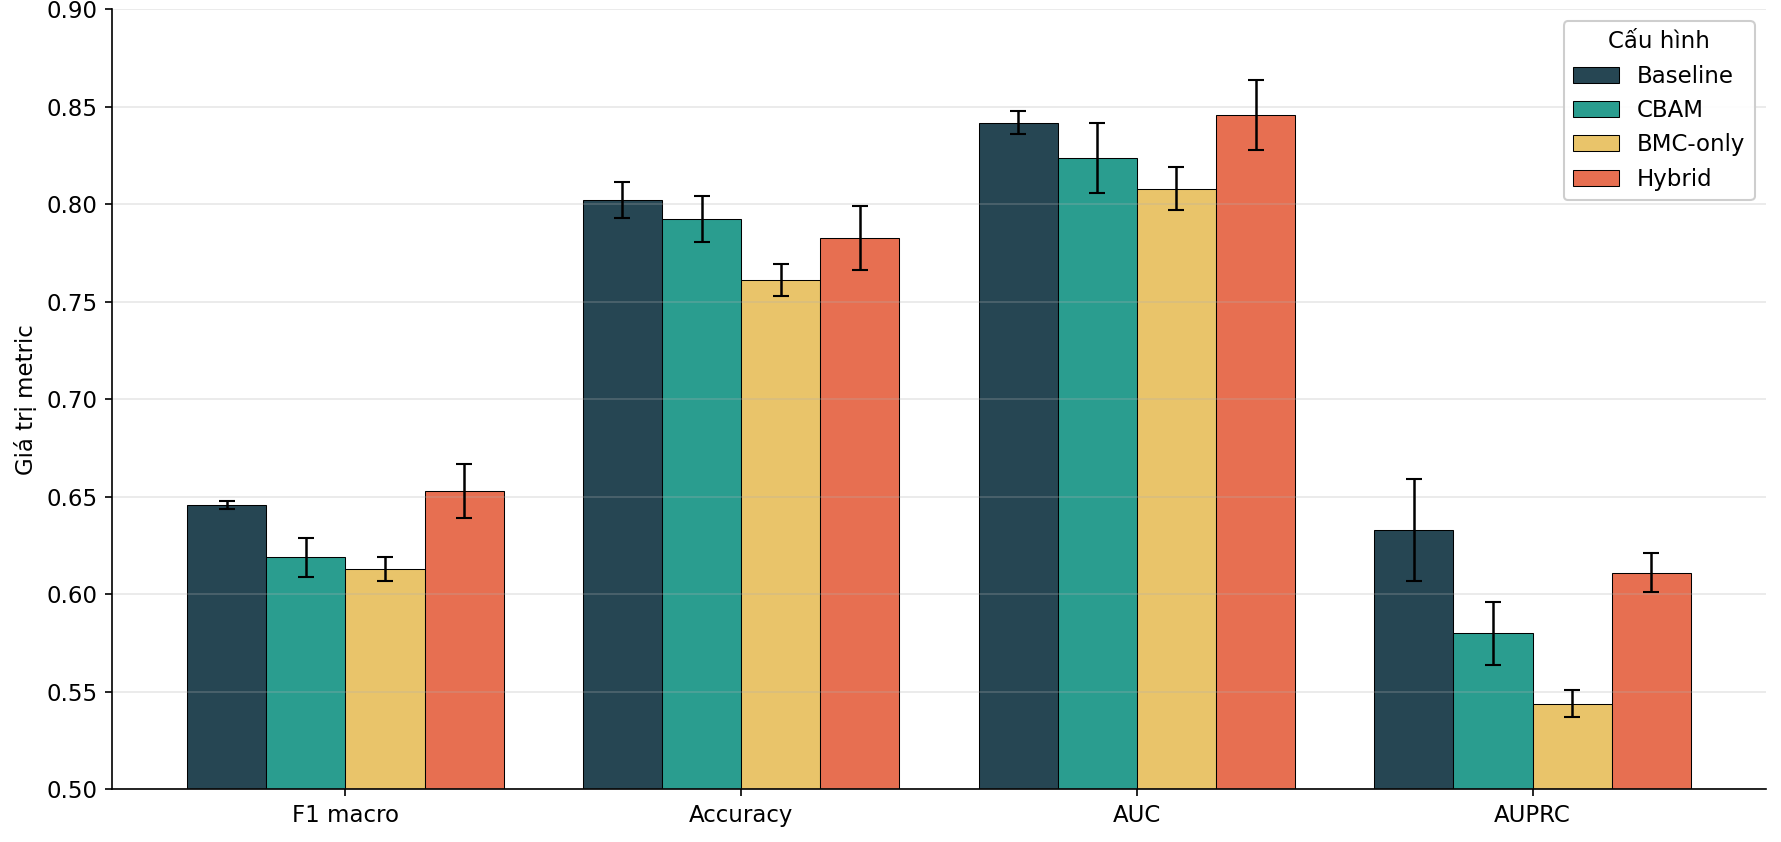
\includegraphics[width=0.95\textwidth]{cslt/spider_3seed_bars.png}
    \caption{SPIDER 8-label: 4 cấu hình $\times$ 4 metrics (3-seed).}
    \label{fig:spider_3seed_bars}
\end{figure}

% \textbf{Finding chính:} CBAM hoạt động \emph{ngược} trên SPIDER --- Mean F1 0.619 thấp hơn SpineNetV2 0.646 (chênh $-0.027$, vượt 2$\sigma$, có ý nghĩa thống kê) dù cải thiện rõ trên RSNA. Hybrid cân bằng tốt cross-dataset: ngang SpineNetV2 về F1 (0.653 vs 0.646, trong noise) nhưng không thoái hóa như CBAM-only. Lý giải: CBAM tinh chỉnh sâu cho phân bố RSNA dễ overfitting khi chuyển dataset; BiomedCLIP frozen trong Hybrid đóng vai trò \emph{regularizer} giúp giữ ổn định. AUPRC có trade-off (SpineNetV2 0.633 dẫn đầu, Hybrid 0.611) --- BiomedCLIP prior cải thiện ranking F1/AUC nhưng làm xáo trộn calibration của xác suất.

Bảng~\ref{tab:spider_per_disease} chi tiết theo từng nhóm bệnh với 6 chỉ số (Acc, Recall, Precision, F1, AUC, AUPRC) cho 3 cấu hình chính (SpineNetV2 / CBAM / Hybrid). Cách tiếp cận hybrid đạt giá trị tốt nhất ở phần lớn các chỉ số, chứng minh đặc trưng ngữ nghĩa của BiomedCLIP kết hợp với ngữ cảnh 3D của CBAM giúp tổng quát hóa tốt hơn trên dữ liệu mới.

\begin{table}[H]
\centering
\caption{Chi tiết SPIDER theo từng nhóm bệnh}
\label{tab:spider_per_disease}
\label{tab:spider_per_disease}
\renewcommand{\arraystretch}{1.15}
\setlength{\tabcolsep}{3pt}
\resizebox{\textwidth}{!}{%
\footnotesize
\begin{tabular}{llccccc}
\toprule
\textbf{Condition} & \textbf{Config} & \textbf{Recall} & \textbf{Precision} & \textbf{F1} & \textbf{AUC} & \textbf{AUPRC} \\
\midrule
\multirow{4}{*}{Modic (4-cls)}
 & SpineNetV2 & 0.374 $\pm$ 0.01 & 0.383 $\pm$ 0.02 & 0.376 $\pm$ 0.01 & 0.731 $\pm$ 0.03 & \textbf{0.545 $\pm$ 0.08} \\
 & CBAM     & 0.370 $\pm$ 0.01 & \textbf{0.385 $\pm$ 0.02} & 0.374 $\pm$ 0.01 & 0.807 $\pm$ 0.05 & 0.463 $\pm$ 0.05 \\
 & BMC-only & \textbf{0.389 $\pm$ 0.01} & 0.377 $\pm$ 0.02 & \textbf{0.381 $\pm$ 0.02} & 0.742 $\pm$ 0.05 & 0.474 $\pm$ 0.03 \\
 & Hybrid   & 0.382 $\pm$ 0.02 & 0.377 $\pm$ 0.01 & 0.379 $\pm$ 0.02 & \textbf{0.827 $\pm$ 0.04} & 0.500 $\pm$ 0.03 \\
\midrule
\multirow{4}{*}{Disc Narrowing}
 & SpineNetV2 & 0.820 $\pm$ 0.00 & \textbf{0.828 $\pm$ 0.01} & 0.823 $\pm$ 0.01 & \textbf{0.927 $\pm$ 0.01} & 0.882 $\pm$ 0.02 \\
 & CBAM     & 0.817 $\pm$ 0.02 & 0.819 $\pm$ 0.01 & 0.818 $\pm$ 0.01 & 0.896 $\pm$ 0.02 & 0.862 $\pm$ 0.01 \\
 & BMC-only & 0.802 $\pm$ 0.00 & 0.789 $\pm$ 0.01 & 0.792 $\pm$ 0.01 & 0.885 $\pm$ 0.01 & 0.829 $\pm$ 0.02 \\
 & Hybrid   & \textbf{0.836 $\pm$ 0.01} & 0.827 $\pm$ 0.01 & \textbf{0.831 $\pm$ 0.01} & 0.916 $\pm$ 0.02 & \textbf{0.884 $\pm$ 0.01} \\
\midrule
\multirow{4}{*}{Spondylolisthesis}
 & SpineNetV2 & 0.597 $\pm$ 0.05 & \textbf{0.793 $\pm$ 0.14} & \textbf{0.632 $\pm$ 0.05} & \textbf{0.826 $\pm$ 0.01} & \textbf{0.325 $\pm$ 0.11} \\
 & CBAM     & 0.500 $\pm$ 0.00 & 0.484 $\pm$ 0.00 & 0.492 $\pm$ 0.00 & 0.822 $\pm$ 0.03 & 0.251 $\pm$ 0.09 \\
 & BMC-only & 0.512 $\pm$ 0.03 & 0.497 $\pm$ 0.02 & 0.501 $\pm$ 0.02 & 0.775 $\pm$ 0.05 & 0.116 $\pm$ 0.04 \\
 & Hybrid   & \textbf{0.633 $\pm$ 0.05} & 0.607 $\pm$ 0.05 & 0.613 $\pm$ 0.04 & 0.815 $\pm$ 0.01 & 0.302 $\pm$ 0.05 \\
\midrule
\multirow{4}{*}{UP Endplate}
 & SpineNetV2 & 0.727 $\pm$ 0.02 & 0.746 $\pm$ 0.02 & 0.728 $\pm$ 0.03 & 0.820 $\pm$ 0.01 & \textbf{0.753 $\pm$ 0.01} \\
 & CBAM     & 0.725 $\pm$ 0.02 & 0.736 $\pm$ 0.02 & 0.729 $\pm$ 0.02 & 0.801 $\pm$ 0.02 & 0.693 $\pm$ 0.03 \\
 & BMC-only & 0.733 $\pm$ 0.01 & 0.724 $\pm$ 0.01 & 0.724 $\pm$ 0.01 & 0.795 $\pm$ 0.02 & 0.698 $\pm$ 0.02 \\
 & Hybrid   & \textbf{0.753 $\pm$ 0.02} & \textbf{0.748 $\pm$ 0.02} & \textbf{0.749 $\pm$ 0.02} & \textbf{0.828 $\pm$ 0.03} & 0.751 $\pm$ 0.03 \\
\midrule
\multirow{4}{*}{LOW Endplate}
 & SpineNetV2 & 0.754 $\pm$ 0.01 & \textbf{0.764 $\pm$ 0.01} & \textbf{0.757 $\pm$ 0.01} & 0.823 $\pm$ 0.02 & \textbf{0.775 $\pm$ 0.02} \\
 & CBAM     & \textbf{0.756 $\pm$ 0.02} & 0.757 $\pm$ 0.02 & 0.757 $\pm$ 0.02 & 0.808 $\pm$ 0.02 & 0.726 $\pm$ 0.03 \\
 & BMC-only & 0.715 $\pm$ 0.02 & 0.711 $\pm$ 0.02 & 0.712 $\pm$ 0.02 & 0.792 $\pm$ 0.02 & 0.709 $\pm$ 0.03 \\
 & Hybrid   & 0.743 $\pm$ 0.04 & 0.745 $\pm$ 0.04 & 0.744 $\pm$ 0.04 & \textbf{0.826 $\pm$ 0.03} & 0.763 $\pm$ 0.03 \\
\midrule
\multirow{4}{*}{Disc Herniation}
 & SpineNetV2 & 0.500 $\pm$ 0.00 & 0.470 $\pm$ 0.01 & 0.485 $\pm$ 0.00 & 0.852 $\pm$ 0.02 & \textbf{0.271 $\pm$ 0.05} \\
 & CBAM     & 0.500 $\pm$ 0.00 & 0.470 $\pm$ 0.01 & 0.485 $\pm$ 0.00 & 0.790 $\pm$ 0.03 & 0.246 $\pm$ 0.04 \\
 & BMC-only & 0.596 $\pm$ 0.07 & 0.556 $\pm$ 0.03 & 0.565 $\pm$ 0.04 & 0.799 $\pm$ 0.02 & 0.183 $\pm$ 0.05 \\
 & Hybrid   & \textbf{0.636 $\pm$ 0.04} & \textbf{0.592 $\pm$ 0.04} & \textbf{0.601 $\pm$ 0.04} & \textbf{0.860 $\pm$ 0.02} & 0.248 $\pm$ 0.10 \\
\midrule
\multirow{4}{*}{Disc Bulging}
 & SpineNetV2 & 0.778 $\pm$ 0.03 & 0.779 $\pm$ 0.03 & 0.777 $\pm$ 0.03 & \textbf{0.874 $\pm$ 0.02} & 0.840 $\pm$ 0.03 \\
 & CBAM     & 0.759 $\pm$ 0.01 & 0.764 $\pm$ 0.01 & 0.758 $\pm$ 0.01 & 0.840 $\pm$ 0.02 & 0.824 $\pm$ 0.03 \\
 
  & BMC-only  & 0.762 $\pm$ 0.01 & 0.768 $\pm$ 0.00 & 0.761 $\pm$ 0.01 & 0.851 $\pm$ 0.02 & 0.834 $\pm$ 0.03 \\
 & Hybrid  & \textbf{0.796 $\pm$ 0.01} & \textbf{0.794 $\pm$ 0.01} & \textbf{0.792 $\pm$ 0.01} & 0.873 $\pm$ 0.01 & \textbf{0.851 $\pm$ 0.03} \\
\bottomrule
\end{tabular}%
}
\end{table}

% \begin{table}[H]
% \centering
% \caption{Recall của các nhãn minority lâm sàng quan trọng}
% \label{tab:spider_minority_recall}
% \renewcommand{\arraystretch}{1.2}
% \setlength{\tabcolsep}{4pt}
% \resizebox{\textwidth}{!}{%
% \begin{tabular}{lccccc}
% \toprule
% \textbf{Condition} & \textbf{Prev. \%} & \textbf{SpineNetV2} & \textbf{CBAM} & \textbf{BMC-only} & \textbf{Hybrid} \\
% \midrule
% Modic Type 1 (rare)        & 0.3\% & 0.000 & 0.000 & 0.000 & 0.000 \\
% Modic Type 3 (rare)        & 0.5\% & 0.000 & 0.000 & 0.000 & 0.000 \\
% Disc Narrowing (Yes)       & 38\%  & 0.758 $\pm$ 0.03 & 0.770 $\pm$ 0.03 & 0.822 & \textbf{0.825 $\pm$ 0.02} \\
% \textbf{Spondylolisthesis Yes} & 3\%  & 0.200 $\pm$ 0.10 & 0.000 $\pm$ 0.00 & 0.056 & \textbf{0.300 $\pm$ 0.10} \\
% \textbf{Disc Herniation Yes}   & 5\%  & 0.000 $\pm$ 0.00 & 0.000 $\pm$ 0.00 & 0.270 & \textbf{0.356 $\pm$ 0.08} \\
% \bottomrule
% \end{tabular}%
% }
% \end{table}
Hybrid dẫn đầu về kết quả của các nhãn thiểu số có ý nghĩa lâm sàng (Disc Herniation, Disc Narrowing), nơi tận dụng được từ các data đã được pretraintd từ BiomedCLIP. Quan trọng hơn, Hybrid là cấu hình duy nhất dẫn đầu cả hai bộ dữ liệu (RSNA lẫn SPIDER khi chuyển tập). Nhánh
BiomedCLIP đóng vai trò chuẩn hóa, giúp mô hình không thoái hóa khi
chuyển sang dữ liệu khác (so với CBAM bị quá khớp với RSNA và thắng rất ít trên SPIDER). Đây là sự cân bằng cần thiết cho triển khai lâm sàng trên nhiều cơ sở y tế khác nhau.
\subsection{Thảo luận chung}
\textbf{Đóng góp methodology:} Báo cáo đã đề xuất kiến trúc Hybrid. Đây là một trong các báo cáo đầu tiên trên cùng dataset có 3-seed mean$\pm$std cho cross-dataset transfer learning.

\textbf{Hạn chế và hướng tiếp theo.} Hướng phát triển sâu hơn được trình bày trong Chương 6.
